%        File: figures.tex
%     Created: Thu Mar 24 12:00 PM 2011 P
% Last Change: Thu Mar 24 12:00 PM 2011 P
%

\documentclass[authoryear, preprint,review,12pt]{elsarticle}
%\usepackage{endfloat}
%\documentclass[final,5p,twocolumn]{elsarticle}
\bibliographystyle{elsarticle-harv}
\usepackage{lineno}
\linenumbers
\usepackage{graphicx}
\usepackage{amsmath,amsfonts}
\usepackage{subfigure}
\usepackage[pdftex]{color}
\definecolor{darkblue}{rgb}{0,0,0.5}
\definecolor{darkgreen}{rgb}{0,0.5,0}
%\usepackage[pdftex, colorlinks, citecolor=darkblue,linkcolor=darkgreen]{hyperref}
\usepackage[pdftex, colorlinks]{hyperref}
\textwidth 6.75in
\oddsidemargin -0.15in
\evensidemargin -0.15in
\textheight 9in
\topmargin -0.5in
\newcommand{\ud}{\mathrm{d}}
\newcommand{\E}{\mathrm{E}}
\newcommand{\C}{\mathrm{Cov}}
\newcommand{\V}{\mathrm{Var}}

%\graphicspath{{/home/cboettig/Documents/ucdavis/research/phylotrees/images/}}

\journal{Nature} 
\begin{document}
\begin{frontmatter}
\title{Quantifying Limits to Detection of Early Warning for Critical Transitions  }
\author[davis]{Carl Boettiger\corref{cor1}}
\ead{cboettig@ucdavis.edu}
\author[davis]{Alan M Hastings}
%\author[davis]{}
\cortext[cor1]{Corresponding author.}
\address[davis]{Center for Population Biology, University of California, Davis, United States}

%\begin{abstract}
%\end{abstract}

%\begin{keyword}
%\sep 
%\end{keyword}
\end{frontmatter}
%\include{figures.tex}
%input{figures.tex}
%\include{body.tex}
%\input{body.tex}


\appendix

\section{The data sets}
All data sets and analyses performed are included in the accompanying R package.
The simulated data sets in Figure 1a of the text are produced with 100 data points
sampled evenly sampled over a time interval (0,100) using the linearized models directly, see~\ref{modelderivations}.
The deteriorating environment was produced under the LSN model~\eqref{LSN}, with $\theta=500$, $\sigma = 5$, $R(t) = 5 - 0.04999 t$.  
The constant data is produced using the simulation method for the constant environment model~\eqref{OU},
with parameters estimated from the deteriorating data-set to correspond as nearly as possible to a similar system. 
The Glaciation data comes from~\citet{Petit1999}, accessible from NOAA:
\href{http://www.ncdc.noaa.gov/paleo/metadata/noaa-icecore-2453.html}{http://www.ncdc.noaa.gov/paleo/metadata/noaa-icecore-2453.html}.
The data is preprocessed by interpoplation and detrending to be as consistent as possible with the analysis presented in~\citet{Dakos2008},
analyzing the third glaciation event. 
The processed data consists of 121 sample points. 
The match is not exact since~\citet{Dakos2008} estimates the de-trending window size manually,
but the estimated correlations in the first-order auto-regression coefficients are in close agreement with that analysis. 
The code for processing the data from the original~\citet{Petit1999} file is included in the accompanying R package.
The Algae example comes from the chemostat ``H6'' in the experiments in \emph{Daphnia magna} populations of~\citet{Drake2010}. 
The analysis in that paper focuses on data averaged over the ensembles, though the supplement includes analysis over individual replicates. 
This individual replicates was chosen as an example of a single replicate 
that showed a statistically significant correlation in variance over window of time where critical slowing down was expected. 
Further empirical examples that have been previously investigated for early warning signs are also analyzed under our approach in~\ref{examples}.   

\section{Averaging over ensembles vs averaging over time}\label{correlations}
The approach of detecting early warning signals by summary statistics is motivated by the ensemble dynamics of a stochastic system.  If we had an infinite number of identical, replicate systems, we could average across replicates to obtain asymptotic estimates of the (for instance) the variance and autocorrelation of the stochastic process $X_t$ at each time $t$, 
\begin{align}
V(X_t) &= \int X_t^2 P(X_t) \ud X_t - \int X_t P(X_t) \ud X_t \\
\text{Autocorr}(X_{\tau}) &= \int (X_t - X_{t-\tau}) P(X_t) \ud X_t 
\end{align}
and so forth for higher moments.  
All of the integrals are over replicates, $X_t$.  
To apply the theory to a single replicate and instead compute the statistics over time windows one must assert that the system is ergodic
--roughly, independent of the time over which it is measured~\citep{Gardiner2009}.  
This cannot be true if the system is experiencing a gradual loss of stability leading to a critical transition -- but may hold  
approximately if the change is gradual relative to the window, and the window is long relative to the relaxation time of the system.
Then if the moments are calculated across the ensemble at sufficiently wide sampling intervals, one may argue that they are approximately independent.  
Only under these assumptions can we apply the approach of summary statistics to a single replicate.  
Even then, we would need techniques from time-series analysis test, 
since we have not satisfied the assumptions of the standard correlations tests.  
Much of the same data are used to compute sequential values of the moments, hence sequential values are temporally correlated.  


This lack of independence violates the assumptions under which the $p$-values associated with typical correlation tests are calculated.
For instance the rank correlations such as Kendall's $\tau$ test a null hypothesis that increases in the $V(X_t)$, etc.
are independent of increases in time, which is not satisfied even when the environment is constant and $X_t$ is stationary.
Calculating $p$-values for Pearson's test needs parametric assumptions such as normal distributed variables as well as independence to define the null distribution.
As both the stationary and the deteriorating environment violate the assumptions of the null, with sufficient data both appear significant.
Consequently the $p$-values seen in Figure 1a and common in the current approaches cannot be interpreted as the probability a warning signal would be observed by chance in a stable system.  

It is possible to define a $p$-value for these correlation statistics by estimating a null distribution consistent with the null hypothesis, as we do through the model-based Monte Carlo estimation of these distributions in Figure 1b of the text, (Type I error).  

\section{Error Types}\label{errortypes}
The $p$-values given in Figure 1a of the text do not correspond to the probabilities 
that the measured value of the statistical test (Kendall's $\tau$) or greater would be observed under a stable system (previous section, \ref{correlations}). 
The approach illustrated in Figure 1b estimates the appropriate null distribution of $\tau$ 
for each warning statistic (variance, autocorrelation, etc.) under the null hypothesis that the system is stable, 
%using Monte Carlo parametric bootstrap approach, section~\ref{parametricbootstrap} 
following the assumption of the stable model defined in the text.\footnote{
While other stable models are possible, this model corresponds to the underlying bifurcation theory behind the design of early warning signals.
Many systems may have dynamics that fall entirely outside the scope of early warning signals~\cite{Hastings2010}. 
Handling such systems as may have dynamics that correspond poorly to any of the models treated here can be addressed by tests of model adequacy, see~\ref{modelchoice}.} 

The appropriate $p$-value for the test statistic can be determined directly from this distribution by integrating to the right of the observed value.
This determines the probability of a false alarm, Type I error.
We are fortunate to be able to estimate the distribution of the test statistic under the alternative hypothesis that the system is stable (red distributions),
and hence can also estimate the power of the test, defined at the accepted false-positive rate.
Having accepted a false-positive rate determines a position beyond which only less than that fraction of the null distribution lies. 
We can ask what fraction of the test distribution lies beyond this fraction as well.
If the false-positive rate is set very low, we lose power. 
The fraction of the test distribution lying to the other side of this accepted rate (1 minus the power) is the probability of a missed event, Type II error.
There is an obvious trade-off between the threshold set for type I error and the resulting Type II error.  

Note that while the Type I error is dependent directly on the value observed in the data (black triangles of Figure 1b \& 1c),
the Type II error depends only on the distributions themselves (though it should be remembered that these are also estimated from the data by means of the model fitting).  

While it is customary in the scientific literature to accept 5\% false-alarm rate,
we emphasize here that this is properly a choice set by management,
under consideration of the relative costs of false alarms and missed events.
In particular, having an estimate of power is very useful in selecting this rate --
if the probability of a missed event is quite high at a 5\% false alarm rate,
it may make sense to use a less conservative estimate of when to act.
We further note that the best management decisions will be based on the probabilities of both outcomes,
rather than forcing a binary decision~\citep{Brozovic2011}.
For this reason we emphasize reporting the entire distributions in Figure 1b \& 1c, rather than only summary information about the error rates.  



\section{Model Derivations}\label{modelderivations}



The sudden collapses we wish to detect are driven by bifurcations when an eigenvalue changes sign in the corresponding deterministic model,
resulting in the sudden loss of a stable state and the onset of a critical transition.
There are many possible models that can contain such a transition.
These may be highly nonlinear models with multiple attractors.
The diversity of possible models can be classified by the type of bifurcation,
such as the saddle-node bifurcation in which a stable point (node) and unstable point (saddle) collide and annihilate,
or a trans-critical bifurcation, in which a stable point becomes unstable.  
(Any dynamical systems textbook, such as \citep{Guckenheimer1983} can give a good overview of such models and bifurcations). 
In general we will be unable to estimate such models accurately if the system has only been observed near the favorable attractor (i.e. before the critical transition occurs),
even if we knew the functional form of the model.  Fortunately the detection of early warning is based on a \emph{local} theory, predicting changes in the dynamics near the current attractor.
Consequently, it is as unnecessary as it is impossible to estimate a fully nonlinear model, but only the linearized model near the bifurcation.

Near the region of the bifurcation,
we can use the simple normal form equation for the bifurcation rather than the full model,
but these are still non-linear and difficult to estimate accurately from the data.
Critical slowing down is based on taking this one step further -- looking at the eigenvalue around the stable point.
This is equivalent to linearizing the normal forms of the bifurcations around the stable point.
By so doing we obtain a simple but general models we can estimate from data.
We are left with explicit, stochastic models that reflect the behavior of the more complicated systems around the stable point, and we can see how they change as they approach the bifurcation.  


\subsection{Saddle-node bifurcation}
The most frequently considered bifurcation model in early warning signals is the saddle-node bifurcation.  
In this bifurcation, a gradual decline is interrupted by a transition when a stable node and saddle node collide and annihilate, 
leaving the system to return to another attractor, if one exists.  
Because this can occur while the system is far from the other attractor, 
this transition appears particularly sudden and has been a focal concern~\citep{Scheffer2001, Scheffer2009}.  

Many models with alternative stable states considered in ecological systems can exhibit this kind of bifurcation.  For instance, a common model is one with a saturating birth rate (such as Holling Type III) and linear death rate, 
\begin{equation}
dX_t = \left( \frac{e K x^2}{X^2 + h_t^2} - e X_t - a_t\right) dt + \sigma \sqrt{ \frac{e K x^2}{X^2 + h_t^2} + e X_t + a_t} dB_t \label{ass}
\end{equation}
This model can experience a saddle-node bifurcation through increased mortality by increasing either $e$ or $a$.  This parameterization is only an example, of course many others are possible~\citep{Scheffer2009a, Scheffer2001, Strogatz2001a, Guckenheimer1983}.  
In this case we have specified the noise dependence on $X_t$ explicitly for the influence of demographic (intrinsic) noise.
The saddle-node bifurcation has normal form
\begin{equation}
\frac{\ud x}{\ud t} = r_t- x^2.
\label{saddle-node}
\end{equation}
Linearizing this model differs from the transcritical bifurcation, since the location of stable point moves as the bifurcation parameter changes.
Transforming the canonical form to allow for an arbitrary mean $\theta$,  the bifurcation looks like $ dx/dt = r_t- (\theta-x)^2 $, with fixed point $\hat x = \sqrt{r_t} +\theta =: \phi$, which gives our second model, LSN: 
\begin{equation}
\ud X = 2\sqrt{ r_t } (\phi - X_t)\ud t + \sigma\sqrt{\phi } \ud B_t. \label{LSN}
\end{equation}


\subsection{Transcritical Bifurcation}
\citet{Drake2010} induce a transcritical bifurcation in laboratory populations of \emph{Daphnia magna} for purpose of testing early warning signals~\citep{Drake2010}. The transcritical bifurcation 

For instance, consider the stochastic Levin's model~\citep{Levins1969} (a logistic model), where $X_t$ is the number of occupied patches of some total number $K$, $c_t$ is a (time-dependent) colonization rate and $e_t$ an extinction rate (both scaled by the number of patches $K$).  
\begin{equation}
\ud X_t = \left( c_t X_t (1-X_t/K) - e_t X_t \right) \ud t + \sigma \sqrt{\frac{e_t}{c_t}} \ud B_t \label{levins},
\end{equation}
such a model can be derived from an individual-based description with or without a stochastic environment, i.e.  \citep{Kampen2007a, Nisbet2004a}.  The model contains a transcritical bifurcation when $c_t < e_t$.  The normal form of the bifurcation is
\begin{equation}
\frac{\ud x}{\ud t} = r_t x - x^2 
\label{transcritical}
\end{equation}

We can rewrite the deterministic part of the Levins model, Eq~\ref{levins} in normal form without loss of generality by taking $r_t = 1 - e_t/c_t$.  
We can linearize around the stable equilibrium value $\hat x(t) = 1 - e_t/c_t = r_t$, 
\begin{align}
\dot x &=  f(x) \approx f'(x)|_{\hat x} (x - \hat x) + \ldots, \\
 &= (r_t - 2 x_t|_{x=\hat x}) (x - \hat x), \\
 &= r_t(r_t - x).
\end{align}
Note the equilibrium time dependence arises not from the internal dynamics but from the changing parameter values.  We can express the linearized stochastic dynamics then by the time dependent mean-reverting process.  We refer to this model as the linearized transcritical bifurcation.  

\begin{equation}
\ud X_t = r_t (r_t - X_t/K) \ud t + \sigma \sqrt{1+r_t} \ud B_t \label{LTC}
\end{equation}

The pattern of the saddle-node differs from that of the transcritical in the square-root dependence on the bifurcation parameter.


\subsection{Modeling limitations}
Many models may differ substantially from~\eqref{ass} and~\eqref{levins} and yet correspond to the linearizations illustrated here.  
The linearizations have thus been constructed with enough free parameters to capture the gross features of the system,
(scaling the equilibrium position, variance, and timescale) while corresponding to the approximations of normal forms of the bifurcations.  
Despite this, there are severe limitations in formulating even a linear approximation without ample knowledge of the system. 
Note that specifying this model such that likelihoods can be calculated still requires a specification of the rate of change of $r_t$.
We assume a linear model,
\begin{equation}
r_t = r_0 - m t
\label{R_t}
\end{equation}
though the approach could easily be extended to an arbitrary model.
A gradual change can be approximately linear over the time interval of interest, and is appropriate to distinguish from a stable model.
Nonlinear rates of change in the environmental conditions will generally be harder to detect (either by summary statistics or the likelihood approach),
thus this assumption is consistent with testing the best case scenario for these methods, illustrating the intrinsic limits of these approaches.  

We also draw attention to the fact that noise scales with the mean dynamics.  
For intrinsically stochastic processes, such as demographic stochasticity, this will scale as the square root, 
while for external perturbations to the system dynamics (environmental stochasticity) this would scale linearly.
We have assumed an intrinsic noise process in both models~\eqref{LSN} and~\eqref{LTC}, 
though an alternative model with linear scaling would also be plausible.  
Note that in these models, the variance observed is determined by the ratio of the Brownian terms (in front of $\ud B_t)$
to the stabilizing force (in front of $\ud t$), so that in general larger $r_t$ will correspond to smaller system variances
regardless of this smaller correction due to the noise scaling with the mean dynamics.  
Either should perform better than the stable model if a system is slowly losing stability,
though using the better-matching model will increase the power of the approach.  

The models here are neither more nor less general than the seemingly model-free approach of summary statistics.  
We have proposed these models to match the assumptions of the summary statistics -- 
that a system is approaching a bifurcation in which a node loses stability as an eigenvalue passes through zero.  


\subsection{Stable Model}
When the system is stable, $r_t$ is constant and both models~\eqref{LSN} and~\eqref{LTC} reduce to a simple Ornstein-Uhlenbeck process, 
\begin{equation}
\ud X_t = r (\theta - X_t) \ud t + \sigma \ud B_t \label{OU}
\end{equation}

\section{Likelihood calculations}\label{likelihood}
The linearization above is not only justified by the nature of and the properties we wish to estimate from the data,
but also convenient for the calculations. 
In particular, the models are specified by linear stochastic differential equations, hence their solutions are Gaussian.
The fundamental challenge is that in modeling a gradual loss of stability, the solutions are also explicitly time-dependent.
Model fitting and comparison requires we can write down the likelihood expression for each model given the time-series data.  

The probability $P(M|X)$ of the data $X$ given the model $M$ is the product of the probability of observing each point in the time series given the previous point and the length of the interval,  
\begin{equation}
\log P(M | X) =  \sum_i \log P(x_i | x_{i-1}, t_i)
\end{equation}
As the processes are Gaussian, the probability density $P$ is normally distributed and we need only calculate its first and second moments.  For the OU process (OU process) this is trivial:

\begin{align}
E(x_i) &= X_{i-1} e^{-r t_i} \theta \left(1 - e^{-rt_i} \right) \\
V(x_i) &= \frac{\sigma^2}{2 r} \left(1 - e^{-2 r t_i} \right)
\label{OUsoln}
\end{align}

For the time dependent models, we have analytic forms only for the dynamical equations of these moments, which we must integrate numerically over each time interval.  This is responsible for most of the computational effort required of this approach.  For the linearized transcritical bifurcation:

\begin{align}
\frac{\ud }{\ud t} E(x_i)&=  r(t)(r(t) - x_i) \\
\frac{\ud}{\ud t} V(x_i) &=  -2 r(t) V(x_i) + (1+r(t))\sigma^2 
\label{LTCsoln}
\end{align}

For the linearized saddle-node bifurcation:
\begin{align}
\frac{\ud }{\ud t} E(x_i)&=  2\sqrt{r(t)}(\sqrt{r(t)}+\theta - x_i) \\
\frac{\ud}{\ud t} V(x_i) &=  -2 \sqrt{r(t)} V(x_i) + \sigma^2 ( \sqrt{r(t)}+\theta )
\label{LSNsoln}
\end{align}

These are numerically integrated using \texttt{lsoda} routine for the likelihood calculation.  

\section{The likelihood statistic}
Likelihood methods form the basis of much of modern statistics, in both Frequentist and Bayesian paradigms.  
The ability evaluate likelihoods directly by computation has made it possible to treat cases that do not conform to traditional assumptions more directly.
The basis of likelihood comparisons has its roots in the Neyman-Pearson Lemma, 
which essentially asserts that comparing likelihoods is the most powerful test
of a choice between two hypotheses~\citep{Neyman1933}, which motivates
tests from the simple likelihood ratio test up through modern model adequacy methods.

The hypotheses considered here are more challenging then the original lemma, as they are composite in nature:
they specify two model forms (stable and changing stability)
but with model parameters that must be first estimated from the data.
Comparing models whose parameters have been estimated by maximum likelihood is first treated by~\citet{Cox1961, Cox1962},
and has since been developed in this simulation estimation of the null distribution~\citep{McLachlan1987}, by parametric bootstrap estimate~\citep{Efron1987}.  
Cox's $\delta$ statistic is simply the difference between the log likelihoods of these maximum likelihood estimates, defined as follows.

Let $L_0$ be the likelihood function for model 0, let $\theta_0 = \arg \max \theta_0 \in \Omega_0$, ($L_0 (\theta_0 |X)$) be the maximum likelihood estimator for $\theta_0$ given $X$, and let $L_0 = L_0 (\theta_0 |X)$; and define $L_1$ , $\theta_1$ , $L_1$ similarly for model 1. The statistic we will use is $\delta$, defined to be twice the difference in log likelihood of observing the data under the two MLE models,
$\delta = -2 (\log L_0 - \log L_1 )$

This approach has since been applied to the problem of model adequacy~\citep{Goldman1993} and model choice~\citep{Huelsenbeck1996}.  
We have extended the approach by generating the test distribution as well as a null distribution, allowing estimate of power and Type II error.  

\section{A note on information criteria}\label{aic}
While it would be possible to compare these models directly by a simple test such as the Akaike Information criterion to compare such models, this would be to attempt to answer the question statistically that should be a management decision -- whether to treat the data as indicative of an impending critical transition -- while leaving unanswered the statistical question of the relative risks of missed events and false alarms.  Using the distributions we compute in Figure 1c, it is easy to assess the performance an AIC-based decision criteria would have, Figure~\ref{aic}.  Without the approach described here, these error rates would be unknown.  Given the distributions, it is clear that the there would be no need to accept the AIC criterion.  For instance, in the empirical data, third panel of Figure~\ref{aic}, it would make sense to use a much more stringent threshold, thereby decreasing the rate of false alarms without any substantial increase in the rate of missed events.  When power of detection is very low such, as in the middle panel, error rates can be particularly high.  Low power could result from only a very gradual loss of power or from inadequate sampling, which can be estimated by comparing parameter distributions, see section~\ref{parameterdistributions}.  


\begin{figure}
\begin{center}
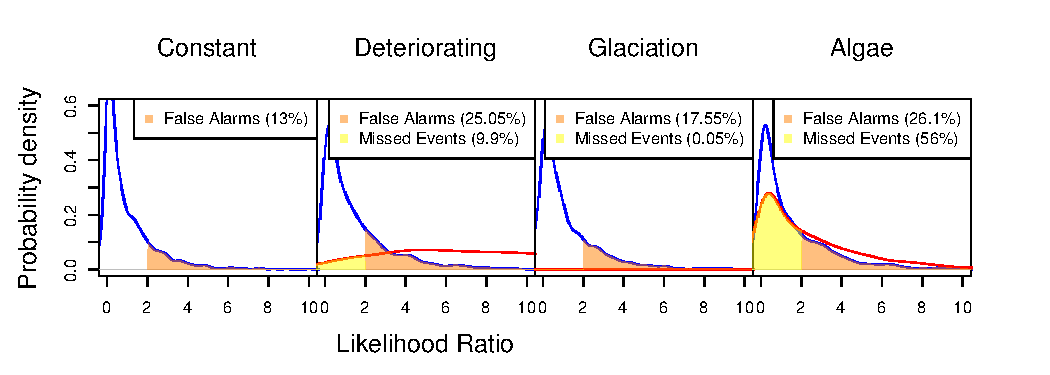
\includegraphics[width=\textwidth]{aic.pdf}
\end{center}
\caption{False alarm and missed detection rate that result from an AIC decision criterion.}
\label{fig:aic}
\end{figure}


\section{Parameter Distributions}\label{parameterdistributions}
% Detecting weak signals
The approach taken in Figure 1c provides a powerful way to indicate when a warning signal can be detected, but more care must be taken with the case in which a signal is not detected.  It will always be easier to say a system is deteriorating (rejecting the null hypothesis that a system is stable) then to establish that a system is stable, as we cannot rule out that we have missed the detection for lack of power.  Thus the left and right panels of Figure 1c make for clear cases of destabilizing systems, while more care must be taken in drawing a conclusion about the middle panel.    

Can we argue that the middle system is truly stable, or could it be experiencing a very gradual loss of stability? The lack of power could be the result of inadequate amount of data or the result of a very gradual change that is difficult to distinguish from  a stable system.  In such cases, the distribution of the estimated stability loss parameter can help establish a lack of power (but potentially rapid rate of stability-loss) from a gradual loss.  Figure~\ref{fig:par} shows an example of this for the case of the simulated loss of stability and the simulated constant environment.  When estimating a changing-stability model on the constant environment data, the distribution for the rate of change is tightly and symmetrically distributed around zero, suggesting that the lack of a signal from this data in the likelihood test is not simply due to a lack of power to detect a very gradual change.  As this data is simulated under a constant environment, this is exactly what we would expect to find given adequate sampling.  

\begin{figure}
\begin{center}
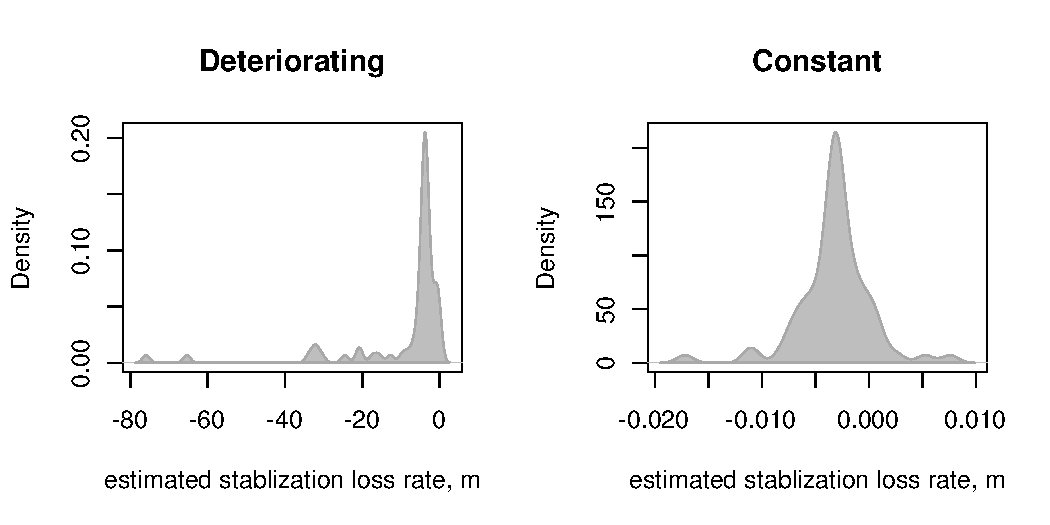
\includegraphics[width=\textwidth]{parameter_dist.pdf}
\end{center}
\caption{.}
\label{fig:par}
\end{figure}

Distributions of all parameter estimates are obtained without extra computational cost by the likelihood approach, and are reported by our package.  Note that this parameter $m$ represents linearized or average rate of loss, and does not preclude the possibility of the rate of deterioration accelerating.  


\section{Model choice and model adequacy}\label{modelchoice}
Any approach is only as good as its underlying assumptions.  In this paper we have leveraged the machinery of likelihood-based approaches to both evaluate the performance of existing methods and provide a statistical test that more closely matches the assumptions of the basic theory.  For this approach to be useful, the data must still be well-approximated by the models used.  We have provided two different simple bifurcation models that could each represent the hypothesis of gradual decline in stability: linearized transcritical bifurcation and the linearized saddle-node bifurcation; Equations~\eqref{LTC},~\eqref{LSN}.  As they both represent a gradual loss of stability either can be used, but the test will be most powerful by using the one that best corresponds to the data.  While knowledge of the system alone can suggest this (such as in the case of~\citet{Drake2010}), it is straight forward to compare the models against each other using the same likelihood framework, as illustrated in Figure~\ref{fig:modelchoice} for several empirical examples.  

\begin{figure}[ht]
\begin{center}
\includegraphics[width=.25\textwidth]{deut_modelchoice.png}
\includegraphics[width=.25\textwidth]{caco3_modelchoice.png}
\end{center}
\caption{Model }
\label{fig:modelchoice}
\end{figure}

As discussed in the text, many systems may not correspond well to any of the simple dynamics upon which the detection of early warning signals is based~\citep{Hastings2010}.  Such dynamics can be particularly misleading for current methods based on summary statistics.  The Monte Carlo bootstrapping of the likelihood approach can be applied as a test of model adequacy, as illustrated in \citet{Goldman1993} and discussed in \citet{Sullivan2005b} in a phylogenetics context. If the observed likelihood ratio falls far from the distributions estimated under either model, the model is likely an inadequate description and subsequent inference may be misleading.  


% Choosing between models

\section{R package tutorial}
We provide an R package with simple implementation of the methods described here.  The package is available from: \href{https://github.com/cboettig/warningsignals/archives/master}{https://github.com/cboettig/warningsignals/archives/master}, where it will be actively maintained and developed.  The package takes an R time-series object (or, for unevenly spaced data -- a matrix or data-frame with sample times in the first column and observations in the second) as input and performs the likelihood analysis illustrated in Figure 1c:

\begin{verbatim}
> require(warningsignals)
>
> # Load a sample dataset
> data(glaciationIII)
>
> # Fit constant (OU) model and a stability-loss model (LSN);
> models <- fit_models(glaciationIII, 'LSN')
>
> results <- montecarlotest(models$const, models$timedep, n=2000, cpu=16)
> plot(results)
\end{verbatim}

The package can generate traditional warning signals (as in Figure 1a) and bootstraps of their uncertainty (as in Figure 1b) for a variety of correlation tests (Pearson's, Kendall's, Spearman's) and summary statistics (variance, autocorrelation, skew) as well.  Copies of data used in the paper are provided as examples.  The Monte Carlo methods can take advantage of multiple core processors or clusters by specifying the number of CPUs in the function argument.   Full documentation of functions and data are provided in the package.  

\section{Examples}\label{examples}
In this section we illustrate the main results of the paper in three further empirical datasets from the climate record.  
\begin{figure}[hb]
\begin{center}
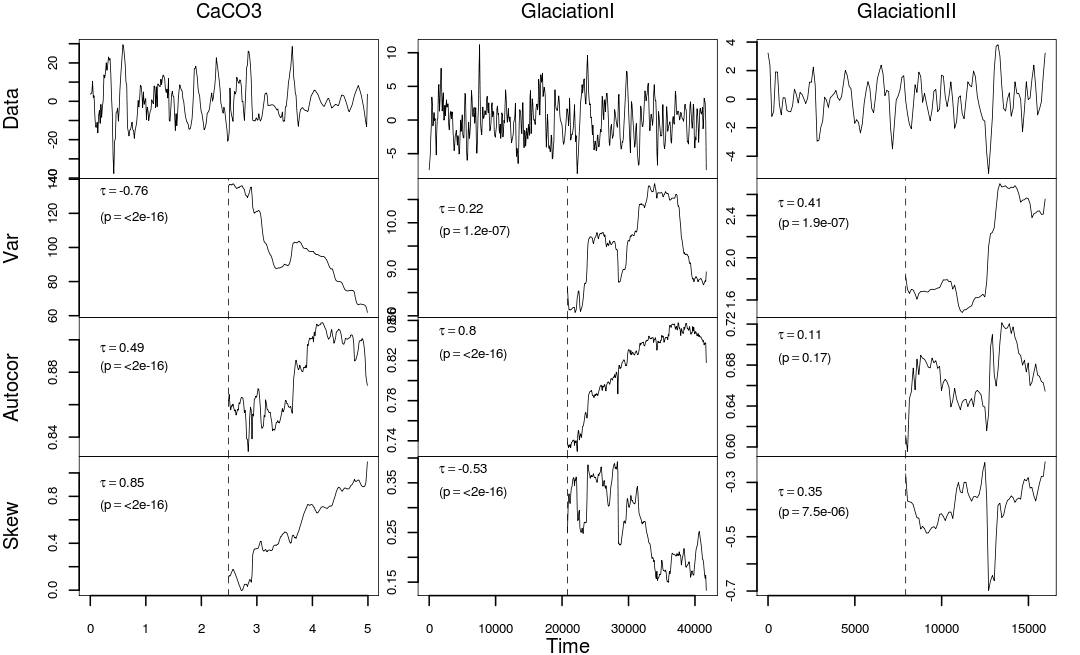
\includegraphics[width=\textwidth]{appendix_fig1}
\end{center}
\caption{Examples for three more empirical datasets from climate records, analysed for warning signals in~\citet{Dakos2008}.  Calcium carbonate data originally from~\citet{Tripati2005}, Deuterium concentrations in the periods before major ice ages from~\citet{Petit1999}.}
\label{fig:1a}
\end{figure}

\begin{figure}
\begin{center}
%\includegraphics[width=.8\textwidth]{figure2_appendix.pdf}
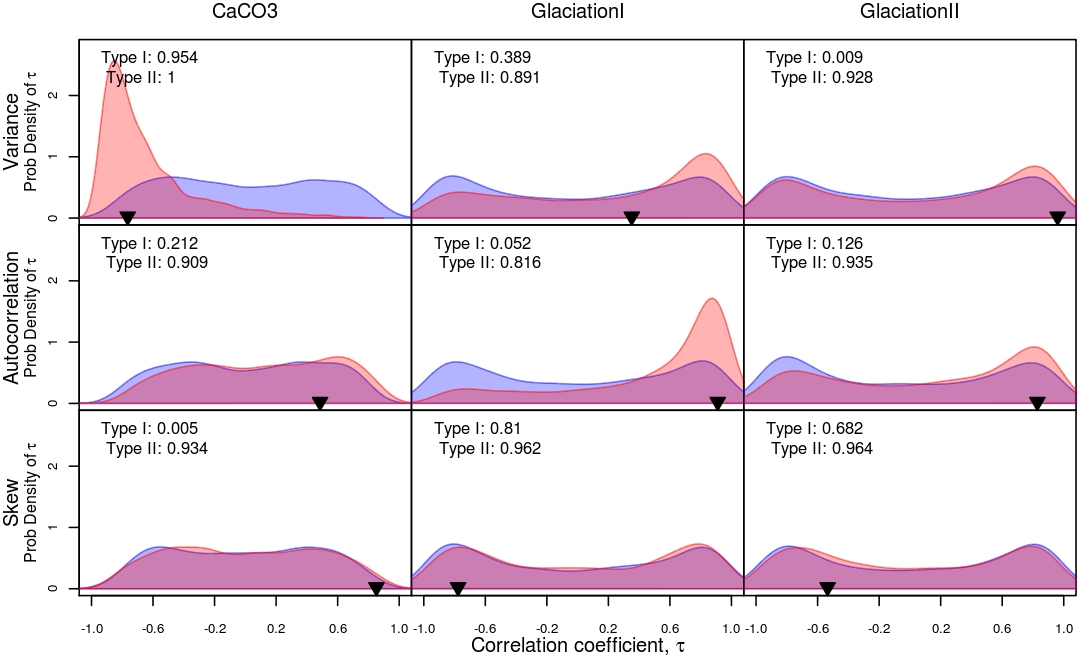
\includegraphics{appendix_fig2}
\end{center}
\caption{Bootstraps of the correlations observed in Figure~\ref{fig:1a}, presented as in Figure 1b in the text.  The distribution of the test statistic under the null (blue) and test (red) hypotheses are difficult to distinguish reliably, across all indicators for each data set.}
\label{fig:1b}
\end{figure}


\begin{figure}
\begin{center}
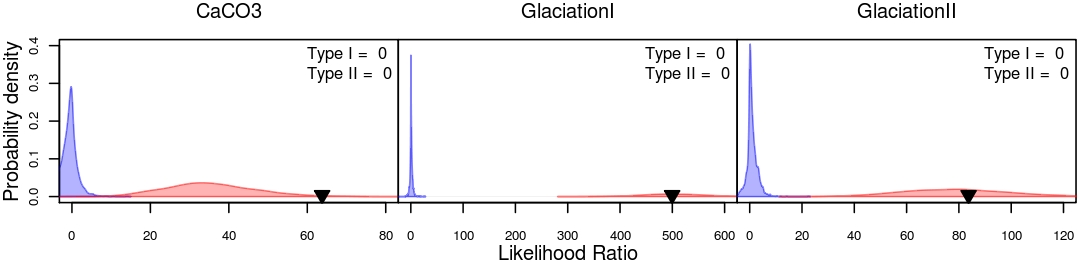
\includegraphics{appendix_fig3}
%\includegraphics[width=.8\textwidth]{figure3_appendix.pdf}
\end{center}
\caption{Bootstraps of likelihood ratios for the data observed in Figure~\ref{fig:1a}, presented as in Figure 1c in the text.  The distribution of the test statistic under the null (blue) and test (red) hypotheses are more clearly distinguished in this approach, supporting the evidence for a warning signal.}
\label{fig:1c}
\end{figure}


\section{Comparisons for additional summary statistics}
Higher moments have also been proposed for the detection of warning signals, such as the skewness~\citep{Guttal2008a}, illustrated for the datasets presented in the text in Figure~\ref{fig:1}.  The skewness appears to have even less power than the other indicators discussed in the text.  

\begin{figure}[ht]
\begin{center}
\subfigure[ ]{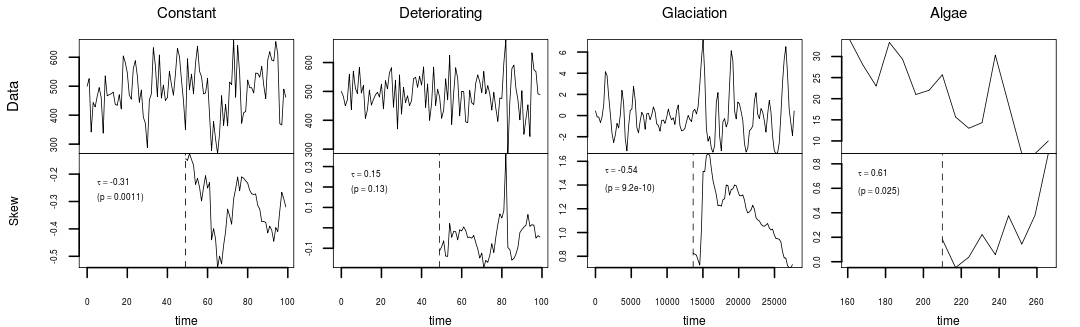
\includegraphics{Boettiger_fig1_appendix.jpg}}
\subfigure[ ] {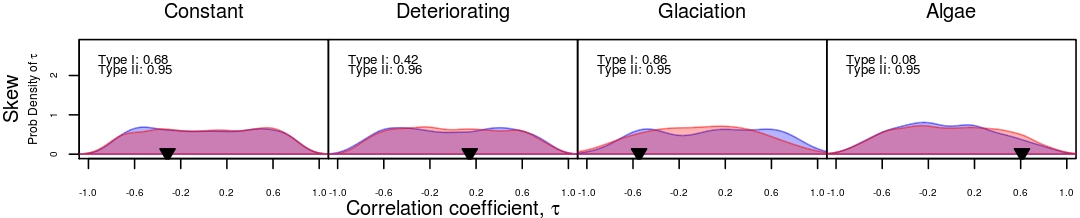
\includegraphics{Boettiger_fig2_appendix.jpg}}
\end{center}
\caption{Increasing skewness is no more likely under the stable hypothesis than the stability-loss hypothesis for each of these data.}
\label{fig:1}
\end{figure}


\pagebreak

\section*{ }%bibliography
\bibliography{/home/cboettig/Documents/bibliographies/library.bib}

\end{document}



